\documentclass[11pt]{article}

\usepackage{fullpage}
\usepackage{newtxtext}
\usepackage[T1]{fontenc}
\usepackage{hyperref,microtype,pdfsync}
\usepackage{amsmath,amsfonts,amssymb,amsthm}
\usepackage{mathtools}
\usepackage{fancyhdr}
\usepackage{algorithm,algorithmic}
\usepackage{graphicx}
%%% BLACKBOARD SYMBOLS

% hyperref package defines C and G, undefined to avoid conflicts
\let\C\relax
\let\G\relax
\newcommand{\C}{\ensuremath{\mathbb{C}}}
\newcommand{\D}{\ensuremath{\mathbb{D}}}
\newcommand{\F}{\ensuremath{\mathbb{F}}}
\newcommand{\G}{\ensuremath{\mathbb{G}}}
\newcommand{\J}{\ensuremath{\mathbb{J}}}
\newcommand{\N}{\ensuremath{\mathbb{N}}}
\newcommand{\Q}{\ensuremath{\mathbb{Q}}}
\newcommand{\R}{\ensuremath{\mathbb{R}}}
\newcommand{\T}{\ensuremath{\mathbb{T}}}
\newcommand{\Z}{\ensuremath{\mathbb{Z}}}
\newcommand{\QR}{\ensuremath{\mathbb{QR}}}

\newcommand{\Zt}{\ensuremath{\Z_t}}
\newcommand{\Zp}{\ensuremath{\Z_p}}
\newcommand{\Zq}{\ensuremath{\Z_q}}
\newcommand{\ZN}{\ensuremath{\Z_N}}
\newcommand{\Zps}{\ensuremath{\Z_p^*}}
\newcommand{\ZNs}{\ensuremath{\Z_N^*}}
\newcommand{\JN}{\ensuremath{\J_N}}
\newcommand{\QRN}{\ensuremath{\QR_{N}}}
\newcommand{\QRp}{\ensuremath{\QR_{p}}}

%%% THEOREM COMMANDS

\theoremstyle{plain}            % following are "theorem" style
\newtheorem{theorem}{Theorem}[section]
\newtheorem{lemma}[theorem]{Lemma}
\newtheorem{corollary}[theorem]{Corollary}
\newtheorem{proposition}[theorem]{Proposition}
\newtheorem{claim}[theorem]{Claim}
\newtheorem{fact}[theorem]{Fact}

\theoremstyle{definition}       % following are def style
\newtheorem{definition}[theorem]{Definition}
\newtheorem{conjecture}[theorem]{Conjecture}
\newtheorem{example}[theorem]{Example}
\newtheorem{protocol}[theorem]{Protocol}

\theoremstyle{remark}           % following are remark style
\newtheorem{remark}[theorem]{Remark}
\newtheorem{note}[theorem]{Note}
\newtheorem{exercise}[theorem]{Exercise}

% equation numbering style
\numberwithin{equation}{section}

%%% GENERAL COMPUTING

\newcommand{\bit}{\ensuremath{\set{0,1}}}
\newcommand{\pmone}{\ensuremath{\set{-1,1}}}

% asymptotics
\DeclareMathOperator{\poly}{poly}
\DeclareMathOperator{\polylog}{polylog}
\DeclareMathOperator{\negl}{negl}
\newcommand{\Otil}{\ensuremath{\tilde{O}}}

% probability/distribution stuff
\DeclareMathOperator*{\E}{E}
\DeclareMathOperator*{\Var}{Var}

% sets in calligraphic type
\newcommand{\calD}{\ensuremath{\mathcal{D}}}
\newcommand{\calF}{\ensuremath{\mathcal{F}}}
\newcommand{\calG}{\ensuremath{\mathcal{G}}}
\newcommand{\calH}{\ensuremath{\mathcal{H}}}
\newcommand{\calX}{\ensuremath{\mathcal{X}}}
\newcommand{\calY}{\ensuremath{\mathcal{Y}}}

% types of indistinguishability
\newcommand{\compind}{\ensuremath{\stackrel{c}{\approx}}}
\newcommand{\statind}{\ensuremath{\stackrel{s}{\approx}}}
\newcommand{\perfind}{\ensuremath{\equiv}}

% font for general-purpose algorithms
\newcommand{\algo}[1]{\ensuremath{\mathsf{#1}}}
% font for general-purpose computational problems
\newcommand{\problem}[1]{\ensuremath{\mathsf{#1}}}
% font for complexity classes
\newcommand{\class}[1]{\ensuremath{\mathsf{#1}}}

% complexity classes and languages
\renewcommand{\P}{\class{P}}
\newcommand{\BPP}{\class{BPP}}
\newcommand{\NP}{\class{NP}}
\newcommand{\coNP}{\class{coNP}}
\newcommand{\AM}{\class{AM}}
\newcommand{\coAM}{\class{coAM}}
\newcommand{\IP}{\class{IP}}

%%% "LEFT-RIGHT" PAIRS OF SYMBOLS

%% NOTE: this requires \usepackage{mathtools} in the document preamble

% inner product
\DeclarePairedDelimiter\inner{\langle}{\rangle}
% absolute value
\DeclarePairedDelimiter\abs{\lvert}{\rvert}
% a set
\DeclarePairedDelimiter\set{\{}{\}}
% parens
\DeclarePairedDelimiter\parens{(}{)}
% tuple, alias for parens
\DeclarePairedDelimiter\tuple{(}{)}
% square brackets
\DeclarePairedDelimiter\bracks{[}{]}
% rounding off
\DeclarePairedDelimiter\round{\lfloor}{\rceil}
% floor function
\DeclarePairedDelimiter\floor{\lfloor}{\rfloor}
% ceiling function
\DeclarePairedDelimiter\ceil{\lceil}{\rceil}
% length of some vector, element
\DeclarePairedDelimiter\length{\lVert}{\rVert}
% "lifting" of a residue class
\DeclarePairedDelimiter\lift{\llbracket}{\rrbracket}
\DeclarePairedDelimiter\len{\lvert}{\rvert}

%%% CRYPTO-RELATED NOTATION

% KEYS AND RELATED

\newcommand{\key}[1]{\ensuremath{#1}}

\newcommand{\pk}{\key{pk}}
\newcommand{\vk}{\key{vk}}
\newcommand{\sk}{\key{sk}}
\newcommand{\mpk}{\key{mpk}}
\newcommand{\msk}{\key{msk}}
\newcommand{\fk}{\key{fk}}
\newcommand{\id}{id}
\newcommand{\keyspace}{\ensuremath{\mathcal{K}}}
\newcommand{\msgspace}{\ensuremath{\mathcal{M}}}
\newcommand{\ctspace}{\ensuremath{\mathcal{C}}}
\newcommand{\tagspace}{\ensuremath{\mathcal{T}}}
\newcommand{\idspace}{\ensuremath{\mathcal{ID}}}

\newcommand{\concat}{\ensuremath{\|}}

% GAMES

% advantage
\newcommand{\advan}{\ensuremath{\mathbf{Adv}}}

% different attack models
\newcommand{\attack}[1]{\ensuremath{\text{#1}}}

\newcommand{\atk}{\attack{atk}} % dummy attack
\newcommand{\indcpa}{\attack{ind-cpa}}
\newcommand{\indcca}{\attack{ind-cca}}
\newcommand{\anocpa}{\attack{ano-cpa}} % anonymous
\newcommand{\anocca}{\attack{ano-cca}}
\newcommand{\euacma}{\attack{eu-acma}} % forgery: adaptive chosen-message
\newcommand{\euscma}{\attack{eu-scma}} % forgery: static chosen-message
\newcommand{\suacma}{\attack{su-acma}} % strongly unforgeable

% ADVERSARIES
\newcommand{\attacker}[1]{\ensuremath{\mathcal{#1}}}

\newcommand{\Adv}{\attacker{A}}
\newcommand{\AdvA}{\attacker{A}}
\newcommand{\AdvB}{\attacker{B}}
\newcommand{\Dist}{\attacker{D}}
\newcommand{\Sim}{\attacker{S}}
\newcommand{\Ora}{\attacker{O}}
\newcommand{\Inv}{\attacker{I}}
\newcommand{\For}{\attacker{F}}

% CRYPTO SCHEMES

\newcommand{\scheme}[1]{\ensuremath{\text{#1}}}

% pseudorandom stuff
\newcommand{\prg}{\algo{PRG}}
\newcommand{\prf}{\algo{PRF}}
\newcommand{\prp}{\algo{PRP}}

% symmetric-key cryptosystem
\newcommand{\skc}{\scheme{SKC}}
\newcommand{\skcgen}{\algo{Gen}}
\newcommand{\skcenc}{\algo{Enc}}
\newcommand{\skcdec}{\algo{Dec}}

% public-key cryptosystem
\newcommand{\pkc}{\scheme{PKC}}
\newcommand{\pkcgen}{\algo{Gen}}
\newcommand{\pkcenc}{\algo{Enc}} % can also use \kemenc and \kemdec
\newcommand{\pkcdec}{\algo{Dec}}

% digital signatures
\newcommand{\sig}{\scheme{SIG}}
\newcommand{\siggen}{\algo{Gen}}
\newcommand{\sigsign}{\algo{Sign}}
\newcommand{\sigver}{\algo{Ver}}

% message authentication code
\newcommand{\mac}{\scheme{MAC}}
\newcommand{\macgen}{\algo{Gen}}
\newcommand{\mactag}{\algo{Tag}}
\newcommand{\macver}{\algo{Ver}}

% key-encapsulation mechanism
\newcommand{\kem}{\scheme{KEM}}
\newcommand{\kemgen}{\algo{Gen}}
\newcommand{\kemenc}{\algo{Encaps}}
\newcommand{\kemdec}{\algo{Decaps}}

% identity-based encryption
\newcommand{\ibe}{\scheme{IBE}}
\newcommand{\ibesetup}{\algo{Setup}}
\newcommand{\ibeext}{\algo{Ext}}
\newcommand{\ibeenc}{\algo{Enc}}
\newcommand{\ibedec}{\algo{Dec}}

% hierarchical IBE (as key encapsulation)
\newcommand{\hibe}{\scheme{HIBE}}
\newcommand{\hibesetup}{\algo{Setup}}
\newcommand{\hibeext}{\algo{Extract}}
\newcommand{\hibeenc}{\algo{Encaps}}
\newcommand{\hibedec}{\algo{Decaps}}

% binary tree encryption (as key encapsulation)
\newcommand{\bte}{\scheme{BTE}}
\newcommand{\btesetup}{\algo{Setup}}
\newcommand{\bteext}{\algo{Extract}}
\newcommand{\bteenc}{\algo{Encaps}}
\newcommand{\btedec}{\algo{Decaps}}

% trapdoor functions
\newcommand{\tdf}{\scheme{TDF}}
\newcommand{\tdfgen}{\algo{Gen}}
\newcommand{\tdfeval}{\algo{Eval}}
\newcommand{\tdfinv}{\algo{Invert}}
\newcommand{\tdfver}{\algo{Ver}}

%%% PROTOCOLS

\newcommand{\out}{\text{out}}
\newcommand{\view}{\text{view}}

%%% COMMANDS FOR LECTURES/HOMEWORKS

\newcommand{\lecheader}{%
  \chead{\large \textbf{Lecture \lecturenum\\\lecturetopic}}

  \lhead{\small \textbf{Theory of Cryptography}\\}

  \rhead{\small \textbf{Instructor:
      \href{http://www.eecs.umich.edu/~cpeikert/}{Chris Peikert}\\Scribe:
      \scribename}}

  \setlength{\headheight}{20pt}
  \setlength{\headsep}{16pt}
}


% VARIABLES

\newcommand{\lecturenum}{6}
\newcommand{\lecturetopic}{PRG Expansion, Blum-Micali}
\newcommand{\scribename}{Alessio Guerrieri}

% END OF VARIABLES

\lecheader

\pagestyle{plain}               % default: no special header

\begin{document}

\thispagestyle{fancy}           % first page should have special header

% LECTURE MATERIAL STARTS HERE

\section{Expanding a PRG}
\label{sec:expanding-prg}

In the last lecture we saw the definition of a Pseudorandom Generator
(PRG) as a deterministic function that, given a seed of size $n$,
outputs a pseudorandom string of length $\ell(n)$.  We can ask the
following question: how big can $\ell(n)$ be?  Is there any limit on
how much pseudorandom data we can generate starting from a seed of a
certain size?  We will find out that if we can get a PRG with even
\emph{one bit} of expansion (i.e., $\ell(n) = n+1$), then we can get a
PRG with \emph{any} polynomial output length.

\begin{theorem}
  \label{thm:prg-expansion}
  Suppose that there exists a PRG $G$ with output of length
  $\ell(n)=n+1$.  Then for any $t(n)=\poly(n)$ (where $t(n) > n$),
  there exists a PRG $G_t$ with output length $t(n)$.
\end{theorem}

\begin{remark}
  The size of the set $\set{G_{t}(s) : s \in \bit^{n}}$ is at most
  $2^n$ (because $G_{t}$ is deterministic), while the number of
  possible $t(n)$-bit string is $|\bit^{t(n)}| = 2^{t(n)}$.  The ratio
  of possible output strings that could actually be output by the PRG
  is at most $2^n/2^{t(n)}= 2^{n-t(n)}$, which is absurdly small when
  $t(n) \geq 2n$ (and even smaller when $t(n) = n^{10}$, say).
\end{remark}

\begin{proof}
  We will construct $G_t(s)$ from $G$.  Our construction will apply
  the function $G(\cdot)$ $t(n)$ times, outputting one new bit at each
  step and reusing the other $n$ bits of the previous step's output as
  a seed.  See the following picture for intuition about the
  construction.

  \begin{figure}[h!]
    \centering
    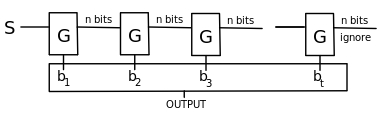
\includegraphics[]{./prg.jpg}
  \end{figure}

  Formally, $G_t$ is defined as follows (note that it always applies
  $G$ on string of the same length, $n$ bits):
  \begin{algorithm}[h]
    \caption{$G_t(s)$}
    \begin{algorithmic}
      \IF{$t = 0$} \RETURN $\varepsilon$ (the empty string)
      \ELSE \STATE let $(x|b)=G(s)$, where $x \in \bit^{n}$, $b \in \bit$
      \RETURN $b|G_{t-1}(x)$
      \ENDIF
    \end{algorithmic}
  \end{algorithm}

  By construction, $|G_t(s)|=t$.  We want to show that $G_t$ is a PRG.
  The function clearly runs in polynomial time (each call to $G$ can
  be resolved in polynomial time and we only use a polynomial number
  of steps), so what's left is to prove that $\set{G_t(U_n)} \compind
  \set{U_{t(n)}}$.  We need to be careful: we already know that $G$ is
  a PRG, but in our construction we are giving a \emph{pseudorandom}
  seed to $G$, instead of a truly random seed.  We will see that this
  fact will not affect the pseudorandomness of $G_t$.  Intuitively,
  because no efficient algorithm can tell a pseudorandom seed apart
  from a random string, then in particular neither can $G$.

  To prove that $G_t$ is a PRG we will define a set of ``hybrid
  experiments.''  We will build a sequence of distributions, where the
  first is equal to our ``real'' construction $G_t(U_{n})$, the last
  is equal to the ``ideal'' truly uniform distribution $U_{t(n)}$, and
  each consecutive pair of distributions are computationally
  indistinguishable.  By the hybrid lemma, we conclude that
  $\set{G_t(U_{n})}$ and $\set{U_{t(n)}}$ are computationally
  indistinguishable and that $G_t$ is a PRG, thus proving the theorem.

  To give some intuition about how we design the hybrid experiments,
  we imagine that instead of invoking the first $G$ on $n$ uniform
  bits, what if we replaced its output with $n+1$ truly uniform bits?
  Intuitively, these two cases should not be distinguishable, because
  $G$ is a PRG.  And then what if we replaced the first two
  invocations of $G$, and so on?  Eventually, we would end up with $t
  = t(n)$ truly uniform output bits, as desired.

  Formally, the hybrid experiments are defined as follows:
  \begin{itemize}
  \item $H_0 = G_t(U_n)$
  \item $H_1 = U_1 | G_{t-1}(U_n)$
  \item In general, $H_i = U_i | G_{t-i}(U_n)$ for $i \in \set{0} \cup
    [t]$
  \item $H_t = U_{t}$
  \end{itemize}

  We now show that for all $i \in [t-1]$, $H_i \compind H_{i+1}$.  We
  will do this by using the simulation/composition lemma, and the fact
  that $G$ is a PRG.  For each $i$, we design a PPT ``simulator''
  algorithm $\Sim_i$ such that $\Sim_i(G(U_n))=H_{i-1}$, and
  $\Sim_i(U_{n+1})=H_i$.  Since we know that $G(U_n) \compind U_{n+1}$
  from the fact that $G$ is a PRG, the composition lemma implies that
  $H_{i-1} \compind H_i$.

  We define $\Sim_i$ as follows:
  \begin{algorithm}[h]
    \caption{$\Sim_i(y \in \bit^{n+1})$}
    \begin{algorithmic}
      \STATE parse $y$ as $(x|b)$ for $x \in \bit^{n}$, $b \in \bit$
      \RETURN $U_{i-1} | b | G_{t-i}(x)$
    \end{algorithmic}
  \end{algorithm}

  This algorithm clearly runs in polynomial time.  We need to check
  that it maps $G(U_n)$ to $H_{i-1}$, and $U_{n+1}$ to $H_i$.  First
  suppose that the input of $\Sim_i$ comes from $U_{n+1}$:
  \[ \Sim_i(U_{n+1})= U_{i-1} | b | G_{t-i}(x) = U_{i-1} | U_1 |
  G_{t-i}(U_n)=U_i | G_{t-i}(U_n) = H_i. \] Now suppose that the input
  comes from $G(U_n)$.  By the definition of $G_t$, we can see the
  following:
  \[ \Sim_i(G(U_n)) = U_{i-1} | b | G_{t-i}(x) = U_{i-1} |
  G_{t-i+1}(U_n)=H_{i-1}. \]
  This completes the proof.
\end{proof}

\noindent To recap, our proof of Theorem~\ref{thm:prg-expansion} took
the following path:
\begin{itemize}
\item We defined a construction: the actual PRG $G_t$ having a
  pseudorandom output of polynomial length.
\item We defined the sequence of hybrid (``imaginary'') experiments.
  In each step, we replaced \emph{one} ``real'' invocation of a crypto
  primitive ($G(U_{n})$) with its ``ideal'' counterpart ($U_{n+1}$).
\item We proved that consecutive pairs of hybrids are computationally
  indistinguishable, using the composition lemma and the security
  properties of the underlying primitives (i.e., that $G$ is a PRG).
  \begin{itemize}
  \item To apply the composition lemma, we defined a
    ``simulator'' (reduction) for each pair of adjacent hybrids and
    analyzed its behavior.
  \end{itemize}
\end{itemize}

\section{Obtaining a PRG}
\label{sec:obtaining-prg}

Thanks to Theorem~\ref{thm:prg-expansion}, we know that all we need is
to obtain a PRG with one extra bit of output.  We describe a
number-theoretic construction, due to Blum and Micali, of such an
object.

\subsection{Number Theory Background}
\label{sec:background}

\begin{theorem}[Euler's theorem]
  \label{thm:euler-thm}
  Let $G$ be a finite abelian (i.e., commutative) multiplicative
  group.  For every $a \in G$, we have $a^{\abs{G}} = 1$.
\end{theorem}

\begin{proof}[Proof of Theorem~\ref{thm:euler-thm}]
  Consider the set $A = a \cdot G = \set{ ax\; :\; x \in G}$.  Because
  $G$ is a group, $a$ is invertible, and we have $A = G$.  Taking
  products over all elements in $A = G$, we have \[ \prod_{x \in G}
  (ax) = \prod_{x \in G} x. \] Because $G$ is commutative, the LHS is
  $a^{\abs{G}} \cdot \prod_{x \in G} x$, and we can multiply by the
  inverse of the RHS to obtain $a^{\abs{G}} = 1$.
\end{proof}


When $G = \Zp^{*}$ for a prime $p$, we have $\abs{\Zp^{*}} =
\varphi(p) = p-1$, so we obtain the following corollary:

\begin{corollary}[Fermat's ``little'' theorem]
  Let $p$ be a prime.  For any $a \in \Zp^{*}$, we have $a^{p-1} = 1
  \bmod p$.
\end{corollary}

The following structural theorem will be very useful.  (Its proof is
elementary bur rather tedious, so we won't go through it today.)

\begin{theorem}
  \label{thm:Zps-cyclic}
  Let $p$ be a prime.  The multiplicative group $\Zp^{*}$ is
  \emph{cyclic}, i.e., there exists some \emph{generator} $g \in
  \Zp^{*}$ such that $\Zp^{*} = \langle g \rangle := \set{g^{1}, g^{2},
    \ldots, g^{p-1}=1}$.
\end{theorem}

\subsection{Discrete Logarithm Problem and One-Way Function}
\label{sec:dlp-owf}

Theorem~\ref{thm:Zps-cyclic} leads naturally to the so-called
\emph{discrete logarithm problem}, which is: given $y \in \Zp^{*}$
(and prime $p$ and generator $g$ of $\Zp^{*}$), find $\log_{g} y$,
i.e., the $x \in \set{1, \ldots, p-1}$ for which $y = g^{x} \bmod p$.
This problem is believed to be infeasible for large values of $p$.

\begin{conjecture}[Discrete logarithm assumption]
  Let $\algo{S}(1^{n})$ be a PPT algorithm that outputs some prime $p$
  and generator $g$ of $\Zp^{*}$.  For every non-uniform PPT algorithm
  $\Adv$, \[ \Pr_{(p,g) \gets \algo{S}(1^{n}), y \gets \Zp^{*}}
  [\Adv(p,g,y) = \log_{g} y] = \negl(n). \]
\end{conjecture}

We would like to design a collection of OWFs based on the discrete
logarithm assumption.  The collection is made up of the functions
$f_{p,g} : \set{1, \ldots, p-1} \to \Zp^{*}$ (for prime $p$ and
generator $g$ of $\Zp^{*}$), defined as \[ f_{p,g}(x) = g^{x} \bmod
p. \] Moreover, these functions are even \emph{permutations} if we
identify $\set{1, \ldots, p-1}$ with $\Zp^{*}$ in the natural way.

It is a tautology that the collection is one-way under the discrete
logarithm assumption.  It is also clear that we can efficiently sample
from the domain of $f_{p,g}$.  But we still need to check that
$f_{g,p}$ can be evaluated efficiently, and that $(p,g)$ can be
generated efficiently.

For the first, we use the standard ``repeated squaring'' technique for
exponentiation, which requires $O(\len{x})$ multiplications modulo
$p$.  The solution to the second issue is not entirely
straightforward.  Given only the prime $p$, it is unknown (in general)
how to find a generator $g$ of $\Zp^{*}$ efficiently.  However, given
the \emph{factorization} of $p-1$, which can be generated along with
$p$, it is possible: every element in $\Zp^{*}$ has order dividing
$p-1$, so $g$ is a generator if and only if $g^{(p-1)/q} \neq 1 \bmod
p$ for every prime divisor $q$ of $p-1$.  The number of non-generators
is at most the sum of $(p-1)/q$ over all prime divisors $q$ of $p-1$,
so the density of generators is typically large enough.  An often-used
special case is $p = 2q+1$ for prime $q$, for which there are $q =
(p-1)/2$ generators.  However, it is not even known whether there
exist infinitely many such ``Sophie Germain'' primes of this form!
(Empirically, though, they are abundant.)

\subsection{Blum-Micali PRG}
\label{sec:blum-micali-prg}

We now present a PRG that uses the ideas presented in the previous
section.  From Section~\ref{sec:expanding-prg} we know that if we have
a PRG that is able to generate one extra bit of randomness, we can
generate a polynomial number of pseudorandom bits.  Our goal will be
the following: we want to construct a PRG $G_{p,g} \colon \Zp^* \to
\Zp^* \times \bit$.\footnote{To be pedantic, $G_{p,g}$ is a
  ``collection'' of PRGs, where the input seed comes from a set that
  depends on the function index $(p,g)$.  It it easy to check that our
  construction from Section~\ref{sec:expanding-prg} is compatible with
  this collection $G_{p,g}$.}

Our solution is a function with the following form: \[ G_{p,g}(x)=
(f_{p,g}(x)=g^x \bmod p \quad, \quad h(x)). \] Note that $f_{p,g}(x)$
performs the modular exponentiation function (which is a one-way under
the discrete log assumption), while $h \colon \Zp^{*} \to \bit$ is
some function (yet to be defined) that provides the additional bit.

Looking at the function, we can make the following observation: if $x
\in \Zp^{*}$ is chosen uniformly at random, then also $f_{p,g}(x)$ is
uniform (because $f_{p,g}$ is a permutation).  We still need to choose
the function $h$, keeping in mind what we want from from the function:
$h(x)$ should ``look like a random bit,'' \emph{even given
  $f_{p,g}(x)$}.  That is, $h(x)$ should compute ``something about
$x$'' that $f$ hides \emph{completely}.

We can think of many possible candidates for $h$: apply the xor
function to all the bit of $x$; take the least significant bit of $x$
(though you will show that this \emph{does not} meet our
requirements!); take the ``most significant bit'' of $x$ (more
precisely, test if $x>\frac{p-1}{2}$).  The last function will be the
one we will use.

Let's formalize the security properties we want from $h(x)$: given
$f(x)$, no algorithm should be able to guess $h(x)$ with much better
than $\frac{1}{2}$ probability.

\begin{definition}[Hardcore predicate]
  \label{def:hard-core-pred}
  A predicate $h: \bit^* \to \bit$ is \emph{hard-core} for $f$ if for
  all non-uniform PPT algorithms $\Adv$,
  \[ \Pr_{x}[\Adv(f(x))=h(x)] \leq \frac{1}{2} + \negl(n). \]
\end{definition}

\emph{Exercise}: Prove that if $h$ is hard-core for a one-way
permutation $f:D \to D$, then \[ (f(x),h(x)) \compind (U(D),U_1), \]
where $x \gets D$.  This means that $G(x)=(f(x),h(x)) \in D \times
\bit$ is a PRG that expands by one bit.

Next time, we will show that under the discrete log assumption, the
``most significant bit'' predicate $h(x) = [x > \frac{p-1}{2}]$ is
hard-core for $f_{p,g}$.

\end{document}

%%% Local Variables: 
%%% mode: latex
%%% TeX-master: t
%%% End: 
